\chapter{Implementation and Evaluation of Capacity Sizing}
\label{chap:permacam}

This chapter considers two sensing applications and the design of wireless sensor systems to achieve the goals of these applications.
We explore the system design for these applications within the context of the conclusions of \cref{chap:intuition,chap:capacity,chap:battery}, which suggest that energy capacity is a first order concern for energy harvesting wireless sensor design.
The first application that we consider is the measurement of fine-grained workplane illuminance. These illuminance measurements are used to inform the operation of a lighting control system to balance artificial and natural light for occupant's workplanes. 
The goals of this application are to measure illuminance at high granularity with high availability and provide a lifetime of at least a decade. 
This application is relatively simple and it is used to validate the simulation and conclusions presented in \cref{chap:intuition,chap:capacity}.
The second application is image-based human occupancy detection and counting. 
Human occupancy measurement can help inform building energy management and climate control.
The goal of this application is to accurately and consistently detect the presence of humans within view while providing a lifetime of several years.
This application considers existing image sensing solutions and reconsiders their design in the context of the conclusions of previous chapters.
This chapter finishes with an examination of the power and energy trends of image-based sensing application requirements and a few predictions for the future of energy harvesting wireless sensor applications and design. 

\section{Measuring Workplane Illuminance}
\label{sec:impl:permamote}

%We discuss the implementation of both the model used to generate the results
%of \cref{sec:store} and \cref{sec:primary}, and the \name hardware that
%is based on these results. All of our hardware and software will be made
%\textbf{open source} for use by other researchers.


\begin{definefigure}{fig:permamote}
    \centering
    \begin{subfigure}{0.7\columnwidth}
        \centering
        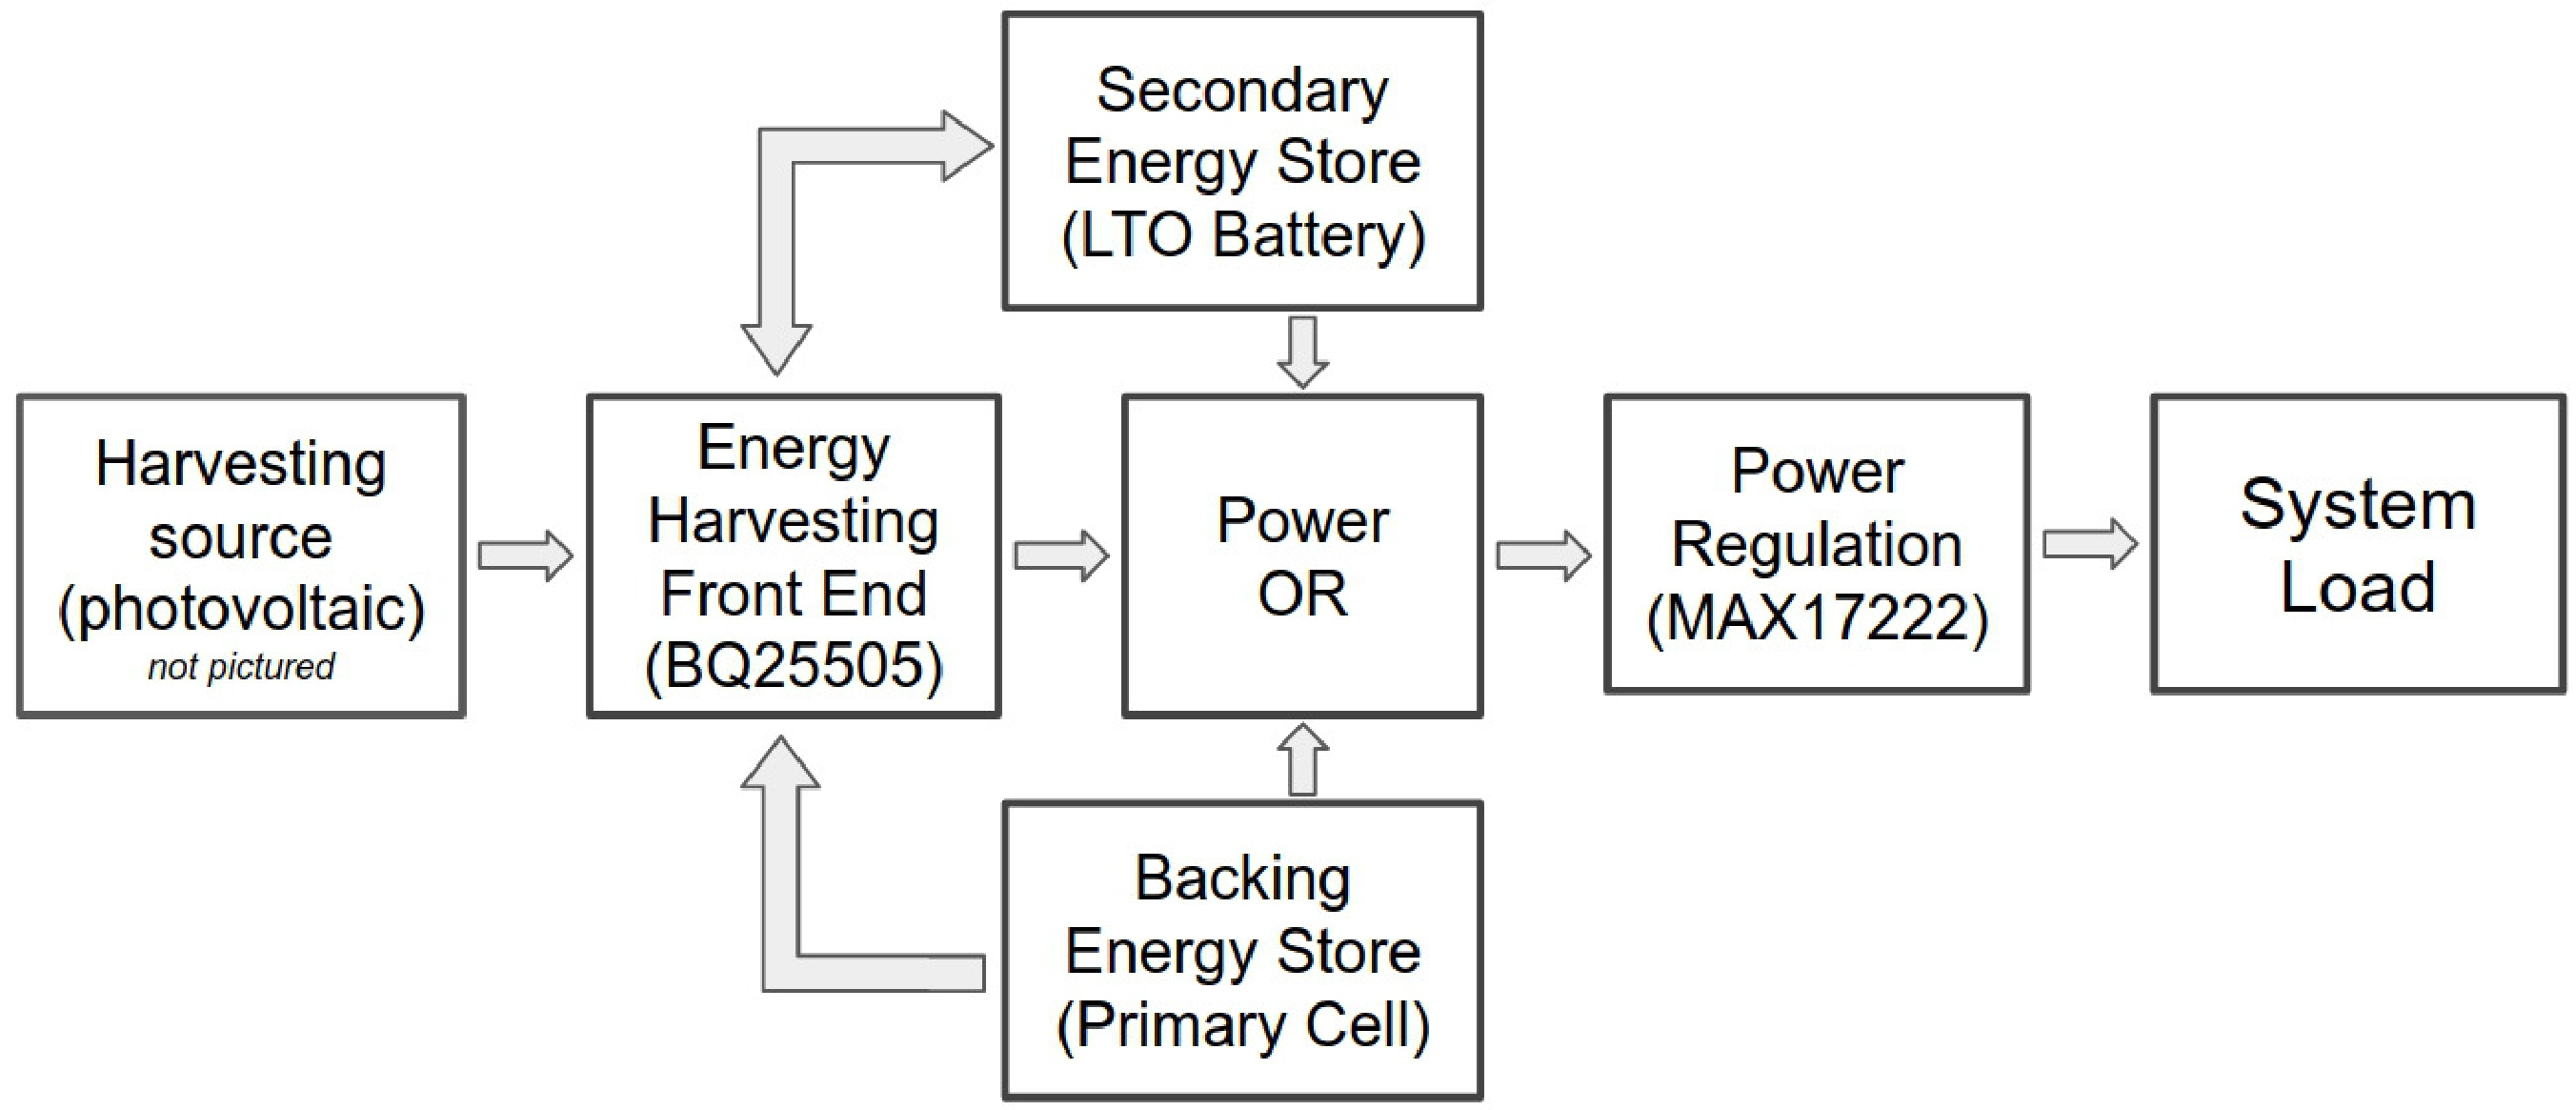
\includegraphics[width=\textwidth]{figs/capacity/arch}
        \caption{Harvesting and storage architecture}
    \end{subfigure}
    \begin{subfigure}{0.29\columnwidth}
        \centering
        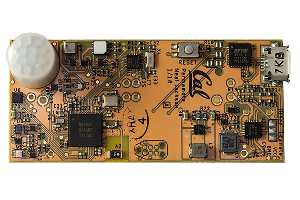
\includegraphics[width=\textwidth,angle=90]{figs/capacity/permamote}
        \caption{Hardware}
    \end{subfigure}
    \caption{\normalfont The \name power supply architecture is informed by the
    findings in \cref{chap:intuition,chap:capacity,chap:battery}. An
    LTO battery is recharged by a solar panel. When the battery is depleted,
    a primary-cell powers the system, providing reliability and avoiding
    intermittency.
    }
    %We believe this platform will run for 6-36 years for common
    %sensing tasks and indoor lighting conditions before the death of
    %the primary-cell. Even after the primary-cell expires,
    %the sensor node could continue to run batterylessly on harvested energy.
\end{definefigure}

The advent of LED lighting has significantly reduced electricity consumption in residential and commercial sectors. However, residential and commercial lighting still consumes 5\% of the \textit{total} U.S. electrical consumption~\cite{aeo2022}.
Beyond the utilization of LED lighting, the technique of daylighting, or lighting buildings with natural light, can further reduce the amount of electricity consumed by buildings. 
Since the intensity of daylight can be unpredictable as it depends on weather, it can be difficult to achieve consistent lighting with natural light alone.
Artificial lighting can be used to augment insufficient natural light, but it requires fine-grained measurement to provide feedback to control and maintain a set point in a space.
In particular, workplane illuminance for commercial buildings is important for occupant comfort and productivity, but is difficult to maintain with existing lighting control systems. 
Modern lighting control systems that perform both measurement and control are generally limited to large zones of measurement and influence. 
The cost of instrumentation and automation is often too exorbitant to justify fine-grained more fine-grained focus.
This often results in inequitable and sometimes uncomfortable lighting for occupants.
Wireless sensing could provide a solution for fine-grained workplane measurement for daylighting applications, assuming the sensor does not require frequent maintenance and provides high availability and consistent measurements for the lighting system feedback loop.
For this specific example, our application goals are to provide at least a ten year lifetime with consistently high availability. 
This section details the realization of a design to meet these requirements, and utilizes this design to verify our the results of the simulation and design conclusions detailed in earlier chapters.

\placefigure{fig:permamote}

\subsection{Design and Implementation}
We design and implement a prototype sensor named \name to perform workplane illuminance sensing based on the application requirements described previously and the design principals discussed in \cref{chap:capacity,chap:battery}.
%The \name sensing platform
%utilizes the components from the representative hardware listed in \cref{tab:capacity:components} 
%used in our simulation. 
\name integrates a processor, BLE/802.15.4 radio, and various environmental, lighting,
and a passive infrared (PIR) occupancy sensor.
The components used in \name are the same ones that we used to develop our representative hardware and workloads for our simulation. 
These components are listed in \cref{tab:capacity:components}. 
A picture
and system diagram of \name is shown in \cref{fig:permamote}. All hardware
and software for the platform is open source\footnote{\url{https://github.com/lab11/permamote/tree/master/hardware/permamote}}.

\subsubsection{Energy Harvesting and Storage.}
Some of the primary goals of \name are to provide workplane illuminance measurements with high availability for a long lifetime of greater than ten years. 
Given the results of our simulation, a design that relies solely on energy preallocation is unlikely to achieve a sufficiently long lifetime. 
\name is powered by an energy harvesting front end that capitalizes on the benefits
of rechargeable and non-rechargeable energy capacity. 
It utilizes the TI BQ25505 energy harvesting IC, which
harvests energy while monitoring both
rechargeable and backup energy stores,
switching between them at user-configurable voltage thresholds~\cite{bq25505}. A
20\ssi{\milli\Ah} (48\ssi{\milli\Wh}) LTO battery is charged by an 10.9\ssi{\centi\meter\squared} amorphous
silicon photovoltaic panel~\cite{LTODatasheet, LTODatasheet2}.
We configure the voltage thresholds of the BQ25505 to derate the 
usable capacity of this battery. This 
increases the apparent cycle lifetime of the battery as described in \cref{sec:battery:life}.
The resulting energy storage provides 24\ssi{\milli\Wh} of
energy storage, more than the capacity required to achieve the reliability and energy utilization
improvements of the workloads that were simulated in \cref{sec:capacity:primary,fig:capacity:primary}.
The chosen photovoltaic panel can provide between an average of 7--70\ssi{\micro\watt} assuming the conservative bounds of indoor irradiance (10--100\ssi[per-mode=symbol]{\micro\watt\per\centi\meter\squared}). 

\placefigure{fig:impl:permamote_life}

\Cref{fig:impl:permamote_life} is a recreation of \cref{fig:capacity:primary} presenting the estimated lifetime of \name with its configured 24\ssi{\micro\Wh} rechargeable storage and various non-rechargeable backup energy storage options.
From this simulation result, \name requires at least one CR2032 coin cell to achieve the application lifetime goals in the worst case energy harvesting potential.
Thus, \name can be configured to either one or two CR2032 coin
cells or a CR123A cell. 
%Primary-cells provide 3-13x more density and 2-12x less
%leakage than a secondary-cell.
%making them more desirable than a single,
%large, pre-charged secondary-cell as the backup store~\cite{LTODatasheet,primary2032, primarycr123a}.
The output of the active battery
is boosted by a MAX17222 regulator, which features high conversion efficiency
(>90\%) at low output currents and operates down to 400\,mV~\cite{max17222}.
%We have the ability to monitor harvesting and system currents using
%the iCount method by sensing the voltage of
%the inductor used by the BQ25505 and MAX17222~\cite{duttaEnergy08}. The processor
%is also capable of gating all sensors from the main power supply to save
%power.\\

\subsubsection{Processor, Radio and Sensor Selection}
In designing \name, we strive to select modern and low power components.
%We feel that it may
To benefit other
platform builders, we document our component selections
along with their key performance metrics. A summary of these
components can be found in \cref{tab:capacity:components}.

We note our choice of the Nordic NRF52840 MCU over the more commonly used MSP430FR series
because of its higher active power efficiency while offering comparable sleep currents.
Specifically, it only draws 56\,\uA/MHz compared to over 100\,uA/MHz
for the MSP430, which is a common choice for batteryless systems. 
Unlike batteryless systems,
\name is designed with sufficient rechargeable capacity and backup energy and is intended to never power off and lose volatile state. 
This eliminates any reliance on state retention techniques and the need for the non-volatile FRAM present on the MSP430FR series chips. 
While
slightly more efficient
processors and radios exist than those found in the NRF52840,
we value the simplicity of the SoC-based design. 

\subsection{Simulation Evaluation using Real Systems}
\label{sec:eval}
To evaluate our simulation and the benefits of a capacity-focused design, 
we perform a three-month-long deployment in a partially sunlit room
using i) a primary-cell only system~\cite{adkins2015michigan}, ii) a batteryless, capacitor-only system~\cite{campbellEnergy14}, and iii) \name, our
system that features both a secondary and primary-cell. 
We model these
systems over the same period using estimated irradiance from \name illuminance masurements. 
We compare the performance and lifetime of these three systems with the predictions generated by a simulation of their workload. 
We also compare the availability of \name to the batteryless system.

%\subsubsection{Simulating Sense and Send with \name}
%We perform benchmarks on the \name platform to develop the workloads presented in \cref{sec:capacity:modelling}.
%The workplane illuminance measurement application represents the same periodic sense and send workload used in our simulation.
%\name requires a total of 586\ssi{\micro\joule} to measure from its light and color sensors and transmit
%the results in a BLE advertisement.
%Out of this event energy, 86\ssi{\micro\joule}
%is required to transmit a single BLE advertisement at 0\,dbm. 
%Additionally, the entire system, including
%the energy harvesting front end, consumes only 5.0\,\uW in deep sleep with volatile state  
%retention and all sensors powered off. 
%We use the energy numbers from \name as a basis
%for our simulation workloads to fairly compare against prior energy storage architectures.

We analyze the deployment of the systems 
%in a partially sunlit room for three months
and compare their behavior to our
model's predictions: i) ten CR2032 primary-cell (720\ssi{\milli\Wh}) only devices, ii) an
batteryless system configured with just 500\textmu F of capacitance (about
0.36\,\textmu Wh at 2.2\,V), and iii) \name, configured with a 20\,mAh
(48\,mWh) secondary-cell, half of which is usable, and a CR2032 backup.  The
primary-cell only device performs environmental sensing over BLE every second.
The batteryless system  sends a beacon as soon as its capacitor bank is full.
When its energy is depleted, it powers off and charges
again. \name is running the ``sense and send'' workload that we described in
\cref{sec:capacity:modelling}, and sends illuminance measurements every second. This
workload stresses the model and requires more charge and discharge cycles.  We
use \name illuminance readings to estimate irradiance using the same scaling factors used by
Yerva et al.~\cite{yervaGrafting12}, and use these traces as
model input for the energy harvesting sensors.

\subsubsection{Primary-Cell Only}
We measure and model the workload of the primary-cell system and produce estimates for
lifetime. The primary cell system requires on average 480\ssi{\micro\watt} to measure and beacon every second. Our model predicts the platform lifetime
to be 58 days.  We find that the average lifetime of the 10 devices is 61 days.
%,
%from initial deployment to energy depletion, is 61 days.

\placefigure{fig:impl:eval_pkt}
\subsubsection{Batteryless}
We model the number of packets sent each hour by the
batteryless system over a three week period, and compare against the results of an actual device in
\cref{fig:eval:pkt}.
Like the simulation of the primary cell system, the model also predicts a more conservative result for the batteryless system. 
The simulation predicts fewer successful packets sent compared to the actual batteryless system under test. 
The average daily error of the model versus our results is 15\%, with a standard deviation of
17\%. This error can attributed to two primary sources. Illuminance is measured
close to, but not exactly at the solar panel of the test device. Occasional
direct sunbeams, like that experienced on day 16, can illuminate the solar
panel but not the sensor, or vice versa. This
results in a substantial over or underestimate of available light. In addition
to inaccurate light measurements, we introduce error through our estimation of
irradiance. We measure illuminance
instead of irradiance, and must resort to a piecewise linear estimation, when
in reality the relationship is not well defined and non-linear when considering
different light sources. In the case of our estimation, results
indicate that the model consistently underestimates high irradiance measurements.

\placefigure{fig:impl:eval_soc}
\subsubsection{Secondary and Primary-Cell}
We compare our model's predicted state of charge to a deployed \name over a seven
day period in \cref{fig:eval:soc}. We estimate state of charge from the reported secondary-cell
voltage,
%,
%and measured voltage
%curves of the installed 20\,mAh battery
and irradiance from
lux measurements. In this figure, the state of
charge cycles between configured battery hysteresis limits, as the workload is
too intense to be sustained by energy harvesting alone.
%and the Permamote must
%use energy from its primary cell.
Flat and upward slopes of the curve represent the
device in hysteresis, using the primary battery to perform its workload. Upper slopes
indicate the secondary cell is charging from harvested energy.
Downward slopes indicate the device is out of hysteresis and is using harvested
energy stored in its secondary battery to perform its workload.
%The device is
%charging and in
%hysteresis during upward
%slopes.
The shaded ``nighttime'' regions are not uniform, as the
deployment environment is occupied by graduate students that occasionally work
late hours or forget to turn off the lights.  The model correctly predicts the
cycling
behavior of the deployed device for two days, but deviates
during the third day. The model predicts that the device would charge above the upper
hysteresis limit and begin supplying energy from the secondary-cell before the
test device actually does.  This inaccuracy, like that of the last of
experiment, is partially due to our inexact estimation of irradiance.  In
addition, real device hysteresis limits are set using resistor networks.  The
resistors used have 1-5\% tolerance, and are susceptible to temperature
changes, which introduces dynamic errors that is not accounted for in our model.
Even though the predicted state of charge deviates after two days, the length
and frequency of periods in which harvested energy is stored and used %in the secondary-cell
are identical to our experimental measurements.
%While our model correctly predicts cycling timing and frequency, it appears the
%state of charge  does not quite match that of the measurements.  This is
%because the voltage measured is not the open circuit voltage, and is affected
%by voltage droop due to the applied system load as well as inflated charging
%voltage from the energy harvesting front end.  Ignoring these effects, the
%cycling of the model's prediction is closely synchronized with the estimated
%state of charge.
%We compare the model's predicted
%state of charge over time to the outputs of systems we
%have deployed. For energy harvesting systems we collect lux measurements
%throughout the deployment and convert lux to irradiance based on the
%data collected in Yerva et al.~\cite{yervaGrafting12}. \\
%\vspace{-6pt}
%\noindent
%\textbf{Permamote.}\\
\subsection{\name Performance and Lifetime}
\placefigure[t]{fig:evalcmp}
\label{sec:eval:permamote}
%In addition to evaluating our model,
We also compare the performance of the
deployed batteryless system and \name. In \cref{fig:evalcmp}, we show the
number of packets sent per hour for two days. \name sends data every
second, while the batteryless system sends as fast as possible. \name is
able to collect and send its data continuously, while the
batteryless system is limited to sending only during the day. This
demonstrates the increased availability afforded by increasing secondary
capacity and including a backup energy store.

We also use our model to explore the estimated performance of \name
compared to the power supply architectures of historical systems for workloads including our illuminance sense and send application and the other applications defined in \cref{sec:capacity:modelling}.
To isolate the analysis to just power supply types and sizing, we assume each
system uses the same low-power hardware and is performing the same workload as \name.
The results of this modeling are shown in \cref{tab:related}. Our model estimates that
\name can expect several decades of 100\% reliable lifetime when configured as
it was deployed for this evaluation, albeit configured with a less intense workload.
%While the workload used with \name is not
%sustainable for the multi-decade lifetimes we are targeting, it still
%exemplifies the increase in reliability afforded by including a primary-cell.

\placefigure{tab:related}

\begin{definefigure}{fig:impl:eval_pkt}
    \centering
    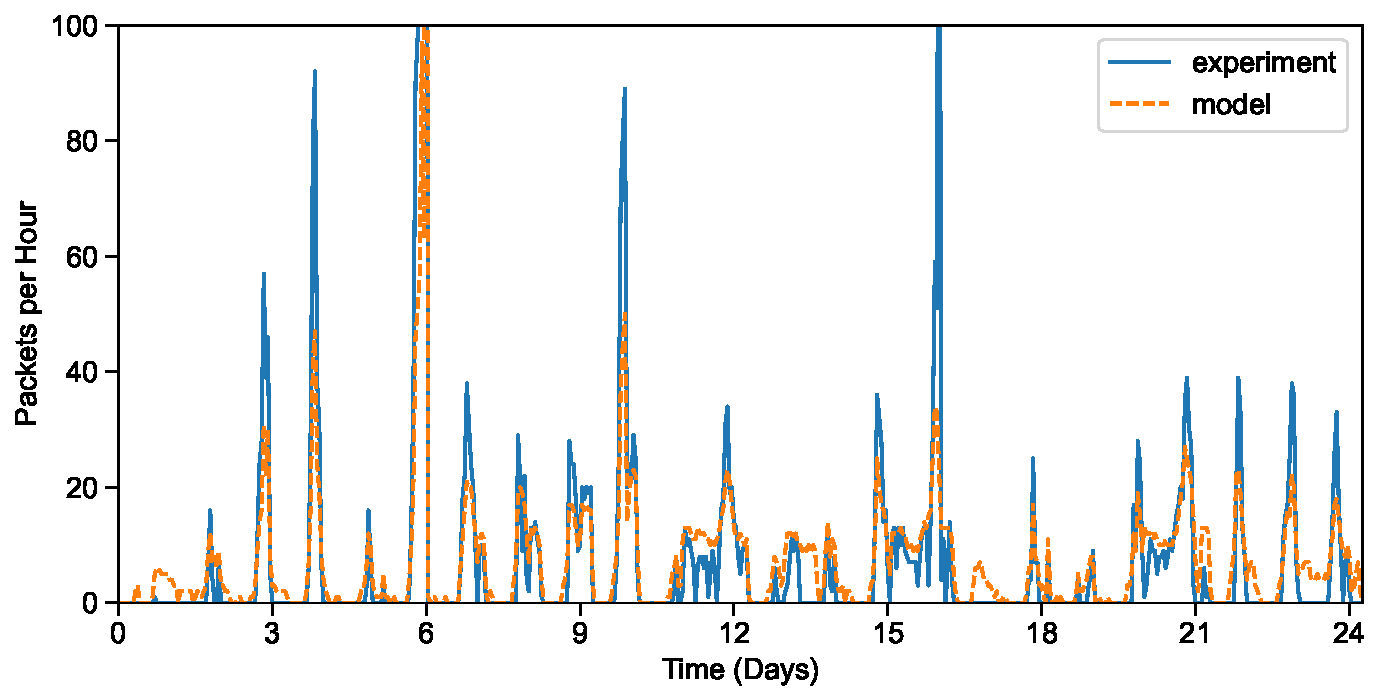
\includegraphics[width=\linewidth]{figs/capacity/experiment_pkt/exp_vs_sim_pkt}
    \label{fig:eval:pkt}
    \caption{Performance comparison of model expectation versus real batteryless system. 
    Data from a three month deployment of two systems is used to verify our model.
    We use three weeks of illuminance measurements %from a month-long deployment
    to estimate irradiance and model the number of packets transmitted by an
    batteryless node. Average daily error is 15\%, with a standard deviation
    of 17\%. 
    } 
\end{definefigure}

\begin{definefigure}{fig:impl:eval_soc}
    \centering
    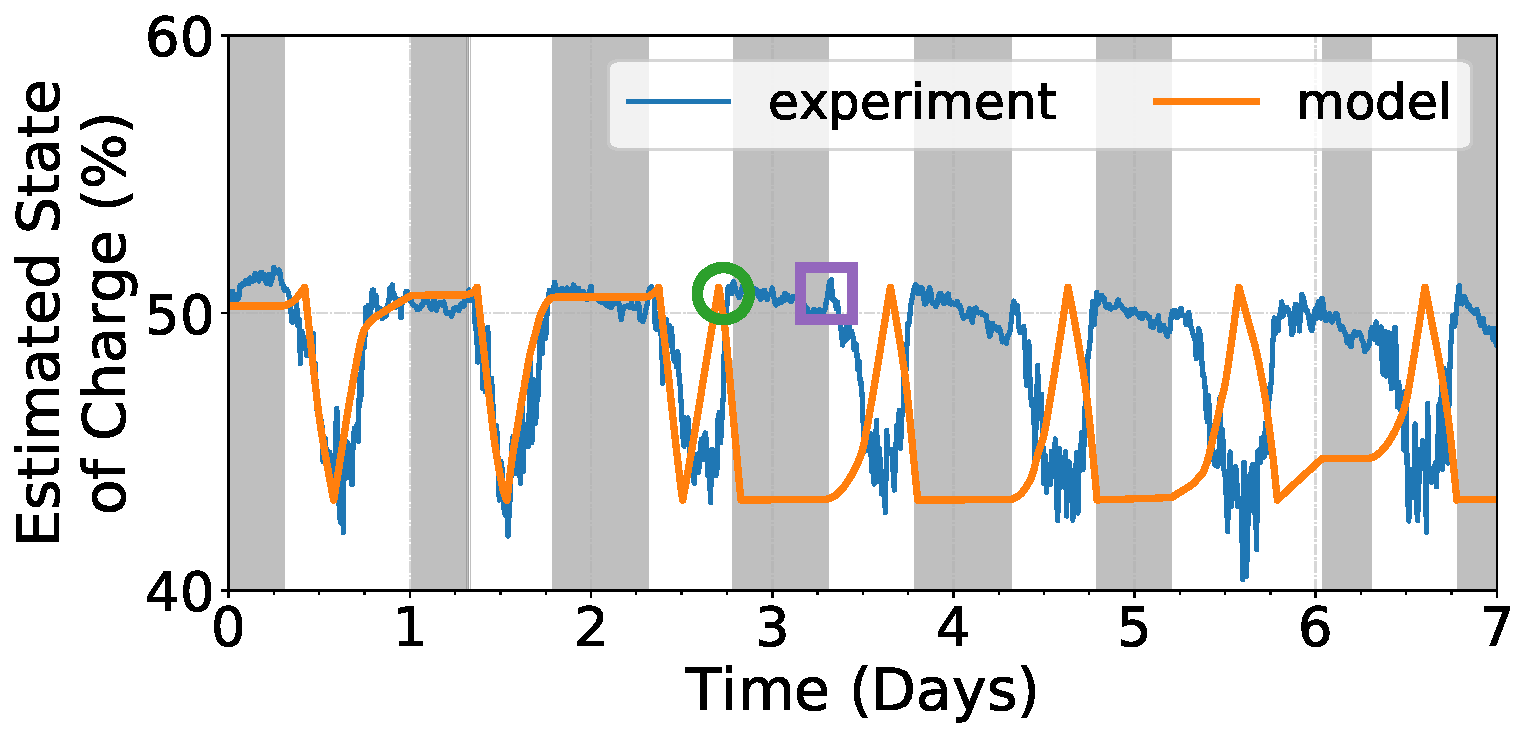
\includegraphics[width=\linewidth]{figs/capacity/experiment_soc/exp_vs_sim_soc}
    \label{fig:eval:soc}
    \caption{The estimated state of charge of a week of a workload compared to our model's estimation.
    We use three weeks of illuminance measurements %from a month-long deployment
    to estimate irradiance and model the number of packets transmitted by an
    batteryless node. Average daily error is 15\%, with a standard deviation
    of 17\%. (b) We model and measure a \name's state of charge while running a
    ``sense and send'' workload with a 1\,s period for a week, beginning at
    midnight on the first day. Charging hysteresis
    limits of the devices are set at 51\% and 43\%. 
    Shaded regions represent periods of low harvestable potential
    (<\,15\,\textmu W/cm\textsuperscript{2}),
    i.e. nighttime. 
    For the first two days, model predictions
    closely track the experimental measurements. Errors
    in hysteresis and irradiance estimation cause the model to reach its upper
    hysteresis sooner than the experiment does, annotated by the
    \textbf{\textcolor{fig-green}{green circle}}. In actuality, the device
    exits charging hysteresis at the peak marked with the
    \textbf{\textcolor{fig-purple}{purple square}}.
    More importantly, the
    frequency and length of periods spent using harvested
    energy collected in the secondary-cell (downward slopes) are identical.
    %For the batteryless node we see our model
    %underestimate the number of transmitted packets by 10-20\% except for the
    %first day which predicts significantly more packets.  We believe this error
    %is primarily due to a piecewise linear estimation of irradiance from our
    %collected illuminance data, when in reality the relationship is complex and
    %non-linear.  For (b) we estimate the state of charge of \name
    %based on the secondary
    %cell voltage. Differences between the estimated state of charge and the
    %modeled state of charge are primarily due to inflated voltage during
    %charging and voltage droop and bounce back when \name
    %draws current from the secondary-cell.
    %Even though estimated state of
    %charge is not accurate due to this voltage swing, it is clear that the
    %timing of charge and discharge aligns between the model and the
    %experimental data.
    }
\end{definefigure}

\begin{definefigure}{fig:evalcmp}
    \centering
    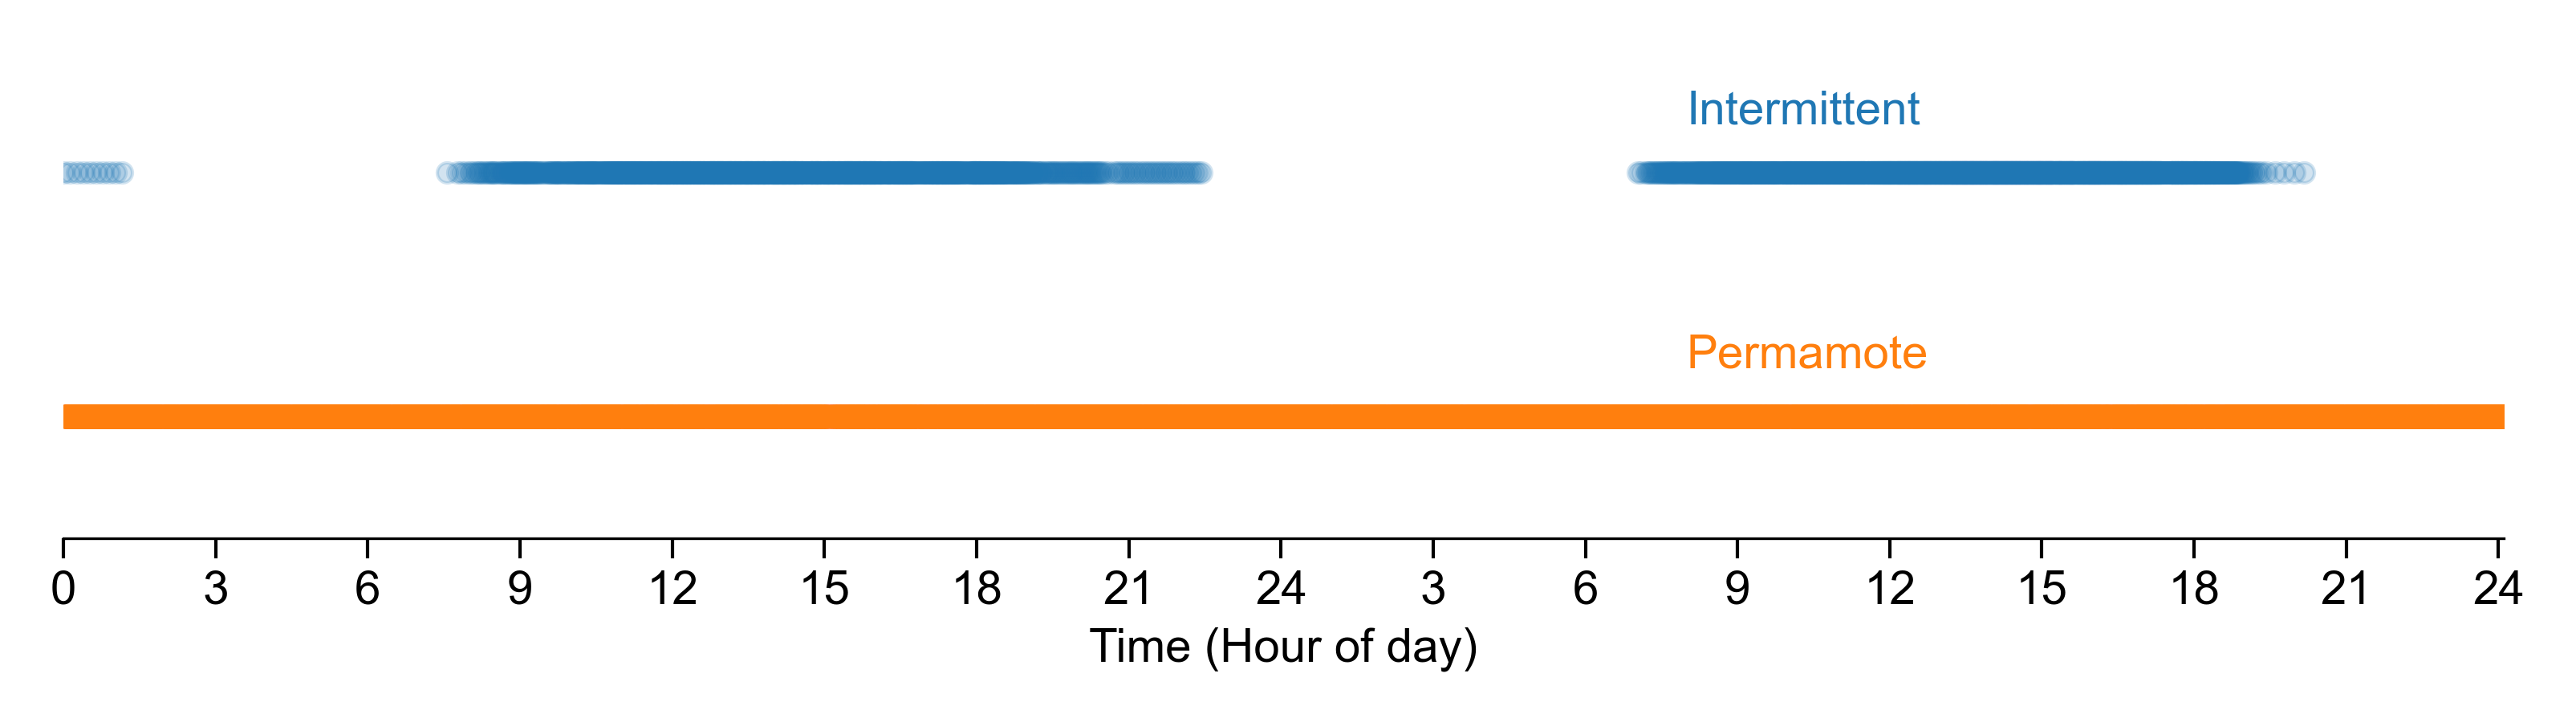
\includegraphics[width=\linewidth]{figs/capacity/experiment_sys_compare/exp_packets_recv}
    \caption{
      \normalfont
        Packets received over two days.
      This figure compares the availability of an
      batteryless design and \name. \name sends a packet every second and does
      so without fail, while the batteryless system is only able to send when
      light is available.
      %This results in periods at night where the
      %batteryless device does not harvest enough energy to sustain operation.
      }
\end{definefigure}

\begin{definefigure}{fig:impl:permamote_life}
    \centering
    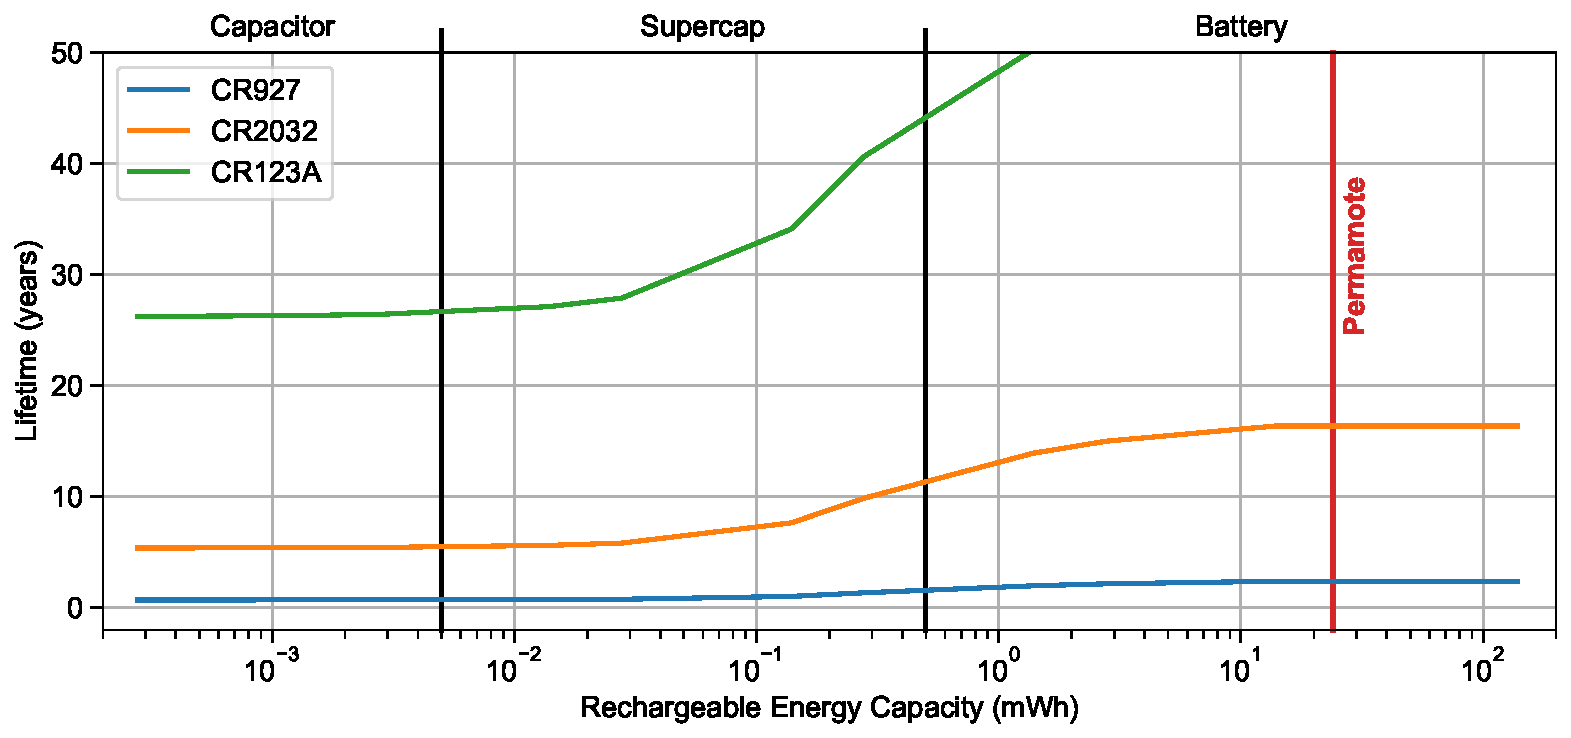
\includegraphics[width=\linewidth]{figs/capacity/primary/sense_and_send_life_vs_sec_size_permamote.pdf}
    \caption{
        Lifetime estimation of the \name sense and send workload given different rechargeable buffer sizes and different primary cell sizes in the low irradiance Setup A environment.
      This is a different presentation of \cref{fig:capacity:primary} that identifies the rechargeable capacity of \name with a red vertical line.
      }
    
\end{definefigure}

\begin{definetable*}{tab:related}
  \begin{threeparttable}
  \centering
  \begin{tabularx}{\columnwidth}{@{\extracolsep{\fill}} l | c c| c c| r}
      \thead[l]{Platform} & \multicolumn{2}{c}{\thead{Successful Events\,(\%)}} & \multicolumn{2}{c}{\thead{Long-Running\\Time to Completion Ratio}} & \thead[r]{Lifetime\\(yrs)}\\
                              & Periodic     & Reactive                     & Average & 95th Percentile & \\
    \hline
    Telos \cite{polastre2005telos}                      & 100   & 100   & 1     & 1     & 8.55\\
    Hamilton \cite{kim2018system}                & 100   & 100   & 1     & 1     & 6.75\\
    BLEES \cite{adkins2015michigan}                     & 100   & 100   & 1     & 1     & 1.11\\
    Gecko \cite{yervaGrafting12}                 & 39.5  & 64.9  & 387   & 981   & $\infty$\,\tnote{g} \\
    Capybara~\cite{colinReconfigurable18}\,\tnote{a}    & 46.3  & 72.8  & 37.6  & 1     & $\infty$\,\tnote{g}\\
    Capybara~\cite{colinReconfigurable18}\,\tnote{b}    & 41.1  & 67.1  & 2730  & 8900 & $\infty$\,\tnote{g}\\
    Flicker \cite{hesterFlicker17}                      & 39.3  & 64.2  & 1307  & 5670 & $\infty$\,\tnote{g}\\
    EnHANTs \cite{margolies2015energy}                  & 79.4  & 96.0  & 1     & 1     & \textemdash\,\tnote{h}\\
    DoubleDip \cite{martin2012doubledip}                & 77.9  & 66.5  & 1     & 1     & \textemdash\,\tnote{h}\\
    \cite{raisigel2010autonomous}                       & 78.4  & 66.9  & 1     & 1     & \textemdash\,\tnote{h}\\
    \textbf{\name}\,\tnote{c}                           & 81.2  & 98.3  & 1     & 1     & \textemdash\,\tnote{i}\\
    \textbf{\name}\,\tnote{d}                           & 100   & 100   & 1     & 1     &  35.8\\
    \textbf{\name}\,\tnote{e}                           & 100   & 100   & 1     & 1     &  30.2\\
    \textbf{\name}\,\tnote{f}                           & 100   & 100   & 1     & 1     &  6.27\\
  \end{tabularx}
    \begin{tablenotes}[para]
      \item[a] With capacitors: 400\,\ssi{\micro\farad} ceramic + 330\,\ssi{\micro\farad} tantalum + 67.5\,mF supercapacitor.
      \item[b] With capacitors: 300\,\ssi{\micro\farad} ceramic + 1100\,\ssi{\micro\farad} tantalum + 7.5\,mF supercapacitor.
      \item[c] No primary-cell.
      \item[d] AA primary-cells like Telos.
      \item[e] CR123A primary-cell like Hamilton.
      \item[f] CR2032 like BLEES.
      \item[g] Lifetimes are theoretically infinite for capacitor-based systems.
      \item[h] Not enough information to predict cycling failure time for theses systems.
      \item[i] Expect cycling degradation in 20-50 years, but do not attempt to estimate.
    \end{tablenotes}
  \end{threeparttable}
  \caption{
  \normalfont
      Modeled performance of energy-harvesting systems.
    For each  platform considered, we model the performance of its energy storage
    architecture. Periodic workload and lifetime estimates are based on a 10\,s
    period, and the reactive workload is scaled to
    generate a maximum of 2000 events per hour (3.4\,s average daily period). Generally,
    intermittent systems have significantly worse availability and responsiveness compared to
    battery-only systems and systems that use a secondary-cell. Battery-only
    systems achieve perfect operation, but have finite, sub-decade lifetimes.
    }
\end{definetable*}

\section{Image-based Person Detection}

\subsection{}


\section{Summary}